%!TEX root = ../dissertation.tex

\chapter{Explainability in Machine Learning}\label{chapt:explainability}

%TODO Altra possibile roba da aggiungere alla intro, da \cite{samek2019xai}.
%In this match AlphaGo played a move, which was
%classified as “not a human move” by a renowned Go expert, but which was the
%deciding move for AlphaGo to win the game. AlphaGo did not explain the move,
%but the later play unveiled the intention behind its decision. With explainable AI
%it may be possible to also identify such novel patterns and strategies in domains
%like health, drug development or material sciences, moreover, the explanations
%will ideally let us comprehend the reasoning of the system and understand why
%the system has decided e.g. to classify a patient in a specific manner or asso-
%ciate certain properties with a new drug or material. This opens up innumerable
%possibilities for future research and may lead to new scientific insights.

In recent years, research on Deep Learning (DL) has achieved remarkable results in a wide variety of domains, going from image recognition, speech recognition, machine translation, playing games, and many others, 
	in some cases even outperforming human capabilities \cite{jumper2021highly, gebru2017using, schrittwieser2020mastering}. 
Although DL is not a new research topic \cite{lecun1989digits,rosenblatt1958perceptron}, its popularity and capabilities skyrocketed only in the last decade: this has been possible mostly thanks to the always growing availability of new data, together with the increase in computational power of modern machines.
Despite the quick and huge success, researchers in the field have already shown some perplexities and moved some critiques towards this approach \cite{marcus2018appraisal,sabour2017dynamic}: is DL really the future of Artificial Intelligence (AI)? Will Neural Networks (NN) be able to give a good approximation of the human brain? Leaving aside such overwhelming questions, we should still be interested in what DL is capable to do at the moment, and what capabilities it still lacks.
One particular aspect for which DL has been criticized is its lack of transparency: in fact, deep models have millions or even billions of learnable parameters, which are not characterizable in any human interpretable way. This results in opaque molearnable e no human supervisor can, ultimately, inteany t what the model has learned by simply inspecting its internal structure. To refer to this undesirable property of deep NNs, the term \say{black box} is commonly used. DL models also present other critical and perplexing issues: in \cite{szegedy2013intriguing} the authors made a neural network misclassify an image by applying an hardly perceptible perturbation, found by maximizing the network’s prediction error. Such adversarial examples have also been found to be somewhat universal and not just the result of overfitting \cite{buckner2020adversarial}. Similarly, authors in \cite{nguyen2015fooled} show how deep neural networks are easily fooled into misclassifying inputs with no resemblance to their true category. This kind of issues pose serious doubts about the ability of NN to learn general representations: indeed, if such networks can generalize well, how can they be confused by what we see as nearly indistinguishable images?  Adversarial examples are not confined to the field of computer vision: natural language networks can also be fooled as shown in \cite{jia2017adversarial,zhang2019generating}. Furthermore, it has been found that in several applications, DL models present strong biasedness. One example is reported in \cite{bolukbasi2016debiasing}, where the authors show how word embeddings trained on Google News articles exhibit strong female/male gender stereotypes due to biases in the training data. Susceptibility to unintuitive errors remains therefore a pervasive problem in DL and no robust solution has been found for them so far. Such issues contribute to generate mistrust, and threaten to slow down or even hinder the prevailance of AI in some applications, due to the high potential of unexpected behavior and lack of verifiability of solutions.
In light of such problems, Explainable Artificial Intelligence (XAI) has become an area of interest in the research community: it tackles the important problem that complex machines and algorithms often cannot provide insights into their behavior and thought processes. The need for XAI is now even more urgent: the renewed EU General Data Protection Regulation (GDPR) could require AI providers to provide users with explanations of the results of ML systems based on their personal data. This clearly affects the industry in a huge way: indeed, the GDPR may hinder or even prohibit the use of \say{black box} models which don't offer explanations for their decisions, when based on users' personal data (think for example to recommender systems). This is also referred to as the \say{right to explanation} \cite{goodman2017european}. The need for XAI has been also expressed by the statement on algorithmic transparency and accountability released by the Association for Computing Machinery \cite{acm2017transparency}, and by the XAI program launched by DARPA in 2017 \cite{gunning2019xai}.

Even though the general aim for XAI is well understood as the achievement of \textit{interpretability}, or \textit{explainability}, for ML models, few articulate precisely what those terms mean or why they are important. In this chapter, we try to provide a more rigorous definition for such terms, by reviewing what has been done in the literature so far. 

\section{Why do we need explainability}
\label{section:whyexpl}
Before determining a good definition for \textit{explainability} or \textit{interpretability}, we must have a good understanding of what the real world objectives of XAI research are. More specifically, what are the desiderata of XAI which are still not being satisfied by the current ML tools and practices. Consider a supervised learning scenario: a lot of evaluation metrics are used to assess the quality of a model, accuracy probably being  the most common one. The computation of such metrics require the presence of model predictions, together with ground truth labels, in order to produce a score which is computed in order to answer in a quantitative way to some questions, like \say{how good is Model A able to generalize with respect to Model B?}, or \say{what is the probability that Model A will misclassify an unseen sample?}. 
This evaluation framework provides satisfactory answers for some kinds of questions, but still fails to answer other ones, especially those demanding qualitative information, with questions like \say{why did the model predict sample $x$ to belong to class $k$?}. 
This kind of questions are the ones sought by XAI research. However, we argue that a rigorous definition for the desiderata of XAI cannot consist in a list of potential questions: this approach is qualitative and already tackled by philosiphical works \cite{bromberger1992we}. We therefore need to express such needs in other forms other than simple questions. 

Lipton \cite{lipton2017mythos} suggests that the need for explainability arises \say{when our real world objectives are difficult to encode as simple real-valued functions}: in this sense, \textit{interpretations} are useful to achieve objectives which are important for us, but which we struggle to model in a formal way. Other mentioned motivating aspects are causality, transferability, informativeness and fair and ethical decision making.
The authors in \cite{doshivelez2017rigorous} refer to this same concept as \textit{incompleteness} in the problem formalization. In such situations, explanations can act as a bridge between the model and the human  supervisor, who can evaluate the predictions based on the provided explanations and decide whether they meet certain criteria that the machine alone could not understand.
 Some examples of such scenarios would be:
\begin{itemize}
	\item \textbf{Scientific Understanding}: humans learn about the world around them in the form of knowledge, which is still difficult to formalize in the same way in which it works inside our brains. For this reason, we might look for explanations from ML models, which in turn we can interpret and transform into human interpretable knowledge.
	\item \textbf{Safety}: in complex tasks, rigorous and complete testing is almost never feasible and it is not possible to formally model all the wrong or dangerous decisions that a model could make. For this reason, when decisions from a ML system can pose a threat to others, explanations can help humans to evaluate safety conditions and to boost trust towards AI.
	\item \textbf{Ethics}: for us humans, evaluating the fairness of a decision is often easy, in the same way in which we have a clear idea of how we would want our model to be ethical (for example, we could desire a \say{fair} classifier for loan approval). However, this kind of properties are not easy to encode in ML systems and, at the same time, biases in the data can often lead to unethical decisions if not treated properly. 
\end{itemize}

Some papers \cite{Kim2015InteractiveAI, ribeiro2016trust} also motivate the need for explainability and interpretability in light of the need for trust by domain experts: indeed trust is fundamental if one plans to act based on a prediction, therefore ML systems must be able to communicate with highly skilled human experts to leverage their expertise and share useful information or patterns from the data. 
%TODO: aggiungi reference a questi papers interessanti a riguardo:
%% Explaining collaborative filtering reccommendations: https://sci-hub.mksa.top/10.1145/358916.358995

%% The role of trust in automation reliance: 
%% https://sci-hub.mksa.top/10.1016/s1071-5819(03)00038-7


\section{When do we need explainability}
Explainability is important in a lot of domains, but not in all of them. There are applications, e.g. aircraft collision avoidance, in which algorithms have been functioning from years without giving any explanations and without any human interaction. It is clear, then, that ML systems can be used without any need for interpretations in real world applications, at least in those cases where their raw performance in terms of accuracy suffices, or when the risk of error doesn't pose any serious threat to the end users. Therefore, domains that demand explainability are generally characterized by the critical nature of decisions which need to be made, where mistakes could have severe consequences. Authors in \cite{burkart2021survey} provide a fairly exhaustive list of domains in need for explainability:
%TODO: think better about how to describe each field
\begin{itemize}
	\item \textbf{Medical Domain/Health-Care}: when the lives of humans are at stake, the need for explanations and knowledge are of paramount importance; take as an example a model used from doctors in order to associate to each patient a risk of suffering a certain disease. Such a model should not only be accurate, but intelligible: in this way, doctors could understand the underlying causes for such a disease, effectively introducing new scientific knowledge in the medical domain;
	\item \textbf{Judicial System}: machine learning systems have also been explored for the automatic decision of judgement results \cite{chen2019judicial}. Such systems should help judges and lawyers to take decisions, but in order to do so their decision must be well motivated;
	\item \textbf{Banking/Finance}: typical examples of automatic decision making in the banking domain are automatic credit approval systems. Since banks are legally obliged to provide customers with motivations when their credit request is denied, the usage of explainable models is required;
%	\item Bio-informatics: 
	\item \textbf{Automobile Industry}: autonomous driving systems are one of the most common and popular applications in DL research. Such autonomous agents are responsible for any accident that could take place on the road: for this reason explanations for each of the agent's decision must be provided, both for legal and security reasons, so that the system can be quickly fixed and improved;
%	\item Marketing
%	\item Election Campaigns
%	\item Precision Agriculture
%	\item Expert Systems for the Military
	\item \textbf{Recommender Systems}: explainable recommendations boost the trustworthiness and effectiveness of recommender systems \cite{zhang2018explainable}. Furthermore, regulations like the aforementioned GDPR are currently requiring models that use users' personal data to provide predictions, to also provide explanations.
\end{itemize}
Examples of other domains requiring explainability include bio-informatics, marketing, election campaigns, precision agriculture or expert systems for the military.
\section{What is explainability}
\label{sec:whatisexplainability}
Several research works attempt to describe rigorously the meaning of explainability in the contest of XAI. In the literature, such word is often used interchangeably or substituted by \say{intrepretability}, even though some try to make a distinction. In \cite{gilpin2018explaining}, for example, the authors claim that explainability is a property of a model that implies interpretability, but not viceversa. More specifically
%, \textit{interpretability} is described as the capability of a certain model to be described in a  way that is understandable to humans; on the other hand, \textit{explainability} is the property of a model to be able to summarize the reasons for their behavior. 
they provide definitions that, we argue, are the most agreed upon in the literature. For clarity, from now on we will interpret those two terms with the following meanings:

\begin{definition}[Interpretability]
	\label{def:interpretability}
	We define \textit{interpretability} in the context of supervised ML as the generic property of a model which makes its individual components, as well as its functioning as a whole, understandable by a human being. Examples of interpretable models are simple linear regression or decision trees. Examples of not interpretable models are deep neural networks.
\end{definition}

\begin{definition}[Explainability]
	\label{def:explainability}
	We define \textit{explainability} in the context of supervised ML as the generic process by which we extract any kind of explanation from a model. This can be done by exploiting the natural properties of the model (in which case, such a model can be called \textit{explainable}), or by devising techniques to extract explanations from any model. 
	
\end{definition}

Explanations, according to the authors, can be evaluated in two ways: according to their intelligibility (that is, its understandability by a human being) and their completeness (that is, the accuracy of the description). Under this definitions, the challenge of XAI is in creating explanations that are both interpretable and complete, even though such characteristics are often opposed to one another. These two features of explanations resemble two important properties of ML models and suggest a similitude: on one hand, the user would desire a simple model with few parameters and at the same time a model able to capture really well the structure of the training data. While both the properties are desirable, they are almost never achievable at the same time. Indeed, as we train simple models, we will probably underfit the data: in the same way, really easy explanations often fail to capture the complexities behind the internal workings of our algorithms. On the other hand, as we add parameters to our model and make it more complex, it will begin to better fit the data: in the same way a really complete explanation will describe accurately the operations of the systems, but will probably result more difficult to understand to a human being. This comparison suggests that, even for explanations, one should allow for a \textit{tradeoff} between interpretability and completeness. The author also suggests that the explanation methods should be evaluated according to how such explanations behave on the curve from maximum interpretability to maximum completeness. This approach is followed in depth in \cite{ribeiro2016trust}, where the authors devise an explanation technique able to work for any classifier, by optimizing the intelligibility-completeness tradeoff. More information about this work is provided in Section \ref{subsec:posthoc}.

%\begin{figure}
%	\centering
%	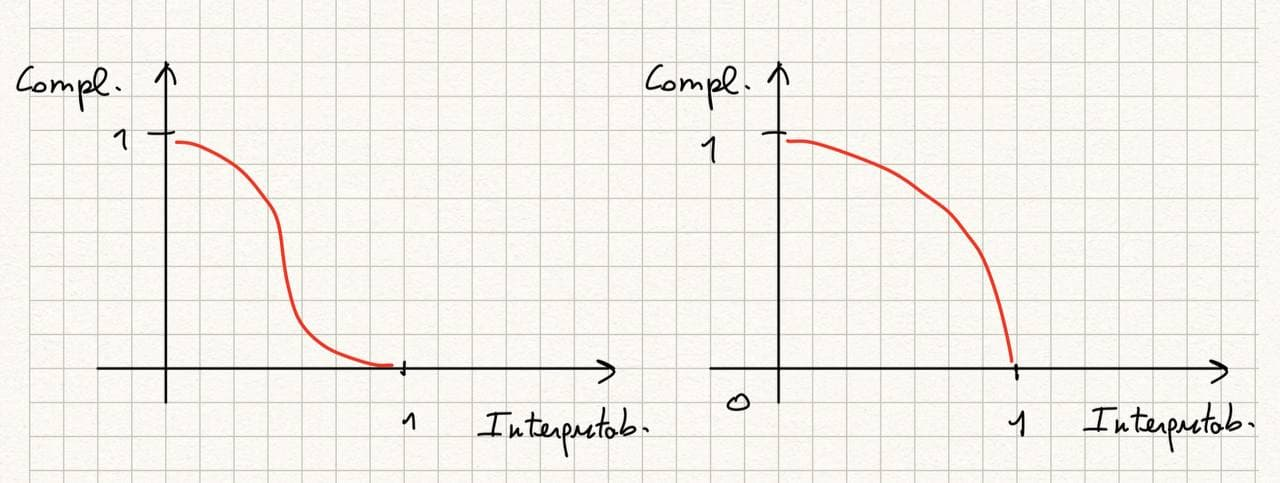
\includegraphics[width=0.9\linewidth]{figures/example_explainability.png}
%	\caption{Example of two different explanations according to the definition given by \cite{gilpin2018explaining}: each explanation allows for a tradeoff between completeness and interpretability. Explanation on the right should be evaluated better than the one on the left: indeed, for higher values of interpretability, the right one offers higher values of completeness.}
%	\label{fig:example_explainability}
%\end{figure}

In \cite{doshivelez2017rigorous} interpretability is defined as the \say{ability to explain or to present in understandable terms to a human}. According to \cite{burkart2021survey}, instead, \textit{interpretability} is most often used in terms of comprehending how the prediction model works as a whole, while \textit{explainability}, in contrast, is used to indicate the capability of models to give explanations about their decision, but keeping their black box nature. In the particular context of generating explanations for DL models, the authors of \cite{montavon2018methods} define an explanation as the collection of features of an interpretable domain (i.e. pixel values on images), that have contributed for a given example to produce a decision (e.g. classification or regression). We can see that none of the aforementioned definitions are specific enough to enable one universal formalization: indeed they implicitly  depend on the context or the aim of the research work. 

Going back to our definitions, we could be tempted to consider an inherently explainable model generally more desirable with respect to an interpretable model. Indeed, interpretability implies an active effort on the part of the human supervisor to dig inside the model, understand the internal mechanisms and infer the model motivations. On the other hand, this process is simplified if the model provides explanations directly, allowing us to immediately have more insights about its decision process. While this may often be true, this certainly does not constitute a rule and, in general, a model can't be said to be interpretable if it is considered explainable, or vice-versa. For example, think about the human brain:
while we are able to give really detailed and motivated reasons behind our decision processes, our brain is not an interpretable model. Indeed, we don't know every single aspect of how our brains works, and yet we (often) trust the explanations that other human beings provide when asked why they took a certain decision. This offers an interesting point of view to the discussion: we should be careful not to trust certain explanations only by the fact that they look plausible and convincing. To this regard, Herman \cite{Herman2017ThePA} warns its readers, making a clear distinction between descriptive and persuasive explanations: indeed implicit cognitive biases of the human brain could mislead us to trust wrong explanations (for example, humans naturally tend to prefer simpler descriptions). To avoid falling in this problem, one should always keep in mind the intelligibility-completeness tradeoff mentioned above.

It is clear that, even after providing some sort of definitions, the meanings of interpretability and explainability are still very generic and slippery. Nevertheless, the volume of research in XAI is quickly expanding, making the number of available methodologies continuously grow. 
%In this work, our interest is mostly towards explainability; in what follows, we focus on reviewing existing techniques for making models explainable.
One fundamental problem in XAI is the definition of specific properties, which make models explainable or interpretable. In the literature, two paradigms are often distinguished \cite{dosilovic2018explainable, lipton2017mythos}: 
\begin{itemize}
	\item \textbf{Transparency}, or integrated interpretability: it is mostly a feature of \textit{interpretable} models. A transparent model can be interpreted by a human thanks to its own easy to understand design. 
	\item \textbf{Post-hoc} interpretability: refers to that approach with which explanations are extracted from already trained models. Such models can be transparent, or retain their black box structure.
\end{itemize}

An intuitive illustration of those two concepts are illustrated in Figure \ref{fig:transparencyvsposthoc}.

\begin{figure}
	\centering
	% TODO: immagine non è proprio corretta
	
\includegraphics[width=\linewidth]{figures/trasparency_vs_posthoc.drawio.png}
	\caption{Intuitive representation of explanations coming from transparent models (left) vs. explanations coming from post-hoc interpretability techniques (right). Transparent models are inherently interpretable by their design; they can be inspected and explanations can be deduced from them. Post-hoc interpretability, on the other hand, refers to a wide range of techniques with which explanations are extracted by any already trained model. }
	\label{fig:transparencyvsposthoc}
\end{figure}

\subsection{Transparency}

Transparency is one of the properties that can enable interpretability and it implies some sort of understanding of the mechanism by which the model works. It can also be seen as the direct opposite to the concept of \textit{black box}. Lipton \cite{lipton2017mythos} goes into even more details, by subdividing transparency in different levels:
\begin{enumerate}
	\item \textbf{Simulatability}: it's the highest level of abstraction of the concept of transparency. Lipton refers to simulatability as the property of the model that makes it understandable by a person \say{at once}. Specifically, this means that a human could, given the input data and all the necessary parameters, produce a prediction by making all the computations in a reasonable time. This notion of transparency is not very applicable to modern machine learning techniques and is often disregarded. 
	\item \textbf{Decomposability}: it's the transparency considered at the level of the single components of the model. Specifically, one model can be considered decomposable if each part of the model (weights, modules, computations...) admits an intuitive explanation.
	\item \textbf{Algorithmic Transparency}: this notion of transparency refers to the learning algorithm itself. For example, we know that in the case of linear regression the shape of the loss function is known, as well as an analytical form for the solution for the problem. This means a maximum degree of algorithmic transparency. On the other hand, modern deep learning lacks this notion of transparency: in fact, even if a lot of powerful optimization algorithms give empirically excellent results, there is no guarantee that those will work on any new problem. The same holds for the shape of the error function, which is almost never known.
\end{enumerate}

It's interesting to notice that the human brain, as noted previously, doesn't exhibit any of those features. In fact, human thinking is not transparent to us and justifications in the form of explanations may differ from the actual decision mechanism. Transparent models are fascinating, but recent research in DL has proven that predictive performances rise when building deeper models, and not vice-versa. For this reason, in recent years, a lot of attention has been put on the research of post-hoc explainability methods.

\subsection{Post-hoc interpretations}
\label{subsec:posthoc}

With post-hoc interpretability we refer to those methods with which we generate explanations from already trained models, without caring about their internal mechanisms. The advantage of this approach is that it does not impact on the performances of the model, which is treated as a black box. Unlike transparency, this kind of interpretability is the one that applies to humans.
%(trovare il modo di parlare di activation maximization... global vs local..., poi ricordarsi di attaccare il discorso difficoltà di integrare prior knowledge)
Lipton \cite{lipton2017mythos} summarizes post-hoc explainability  methods into 
%four main categories: text explanations, visualizations, local explanations and explanations by example.
the following categories.

%\subsubsection{Text explanations}
%This approach aims to mimic the way humans provide explanations to one another, that is, in text form. Example of such approaches: in reinforcement learning \cite{krening2017leaning}, in recommender systems: 
%\cite{mcauley2013hidden} 
%
%\textcolor{red}{(Non ho ancora trovato molti esempi di metodi di questo tipo, forse la tolgo come categoria)}

%TODO: search other examples and refine...


\subsubsection{Visualization}
Another popular approach for post-hoc interpretations is to provide visualizations in order to have a qualitative idea of what the model has learned. For example, when models learn embeddings in high dimensional vector spaces, one popular technique to visualize them is t-SNE \cite{laurens2008tsne}, which provides 2D or 3D visualization of high dimensional data points, in such a way that nearby samples are likely to appear closer together. In the field of computer vision, several papers have investigated the internal representations of visual concepts in CNNs. In \cite{mordvintsev2015inceptionism}, the authors try to build \say{prototipes} of certain objects starting from already trained image classification models. Specifically, starting from a white noise image, they tweak it in such a way that the activation of a certain neuron (in this case, the output neuron corresponding to the selected object) is maximized. This process can be replicated also starting from an existing image, a process which produces really peculiar visual effects (see Figure \ref{fig:image_dream_map}). 

\begin{figure}[h]
	\centering
	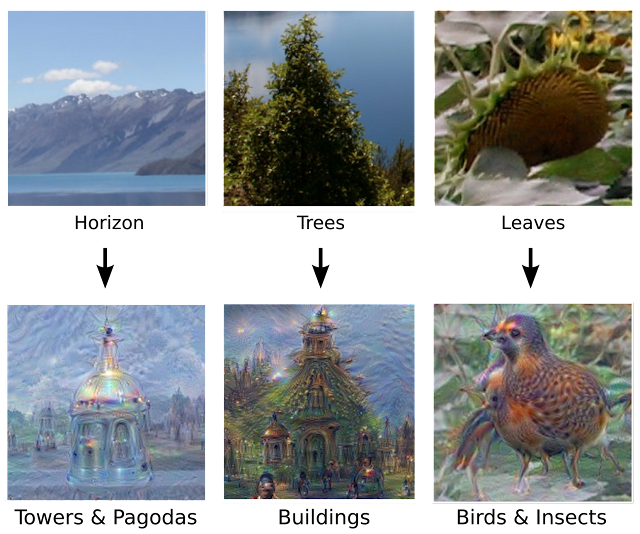
\includegraphics[width=0.6\linewidth]{figures/image-dream-map.png}
	\caption{Process of image manipulation shown in \cite{mordvintsev2015inceptionism}. From an intuitive point of view, starting from existing real images, the network is asked to enhance the features of the image that resemble the desired object (in this case, starting from an image of a tree, start looking for features that resemble buildings). This process is then repeated, creating a positive feedback loop. As a result, the features of the desired objects appear seemingly out of nowhere.}
	\label{fig:image_dream_map}
\end{figure}

This process is also known as \textit{Activation Maximization}: consider a deep NN classifier which maps an input tensor (in this case an image) $x$ to a set of classes $\{\omega_i\}_{i=1}^m$. In a classification scenario, we know that the $i$-th output neuron encodes the modeled class probability $p\left(\omega_i|x\right)$. The basic idea is that the \textit{prototype} $x_i^*$, representative of class $\omega_i$ can be found as follows:

$$x_i^* = ´\max_x \log p(\omega_i|x) - \lambda \|x\|^2.$$

The proposed definition doesn't yield good results in practice: although producing strong class response, they often look unnatural. This problem is solved in several ways, for example by adding regularization via a data density model, or imposing prior constraints which are common in real images, such as high correlation among neighboring pixels. Again, a similar approach is found in \cite{mahendran2014understanding}, where the authors investigate the amount of information retained in the hidden representations of CNNs. They manage to reconstruct the original images with good accuracy even from high level representations by performing gradient descent on white noise inputs.

\subsubsection{Local explanations}
 With visualization techniques, one aims to understand what the model learned from a global point of view: for example, the activation maximization technique described earlier will reflect the \say{internal representation} that the model has of a particular class. With local explanations, instead, one aims at giving explanations in the context of a specific example. One popular approach is the computation of saliency maps, or relevance scores \cite{simonyan2013deep, montavon2018methods, wang2016dueling}. Specifically, given a data point $x \in \mathbb{R}^k$, and given the learned function $f$, the predicted class for point $x$ will be $f(x)$; this approach aims to assign to each feature a score $R(x)_ i$, representing a measure of how relevant the feature $x_i$ is for explaining $f(x)$. One simple approach to obtain the relevance scores is \textit{sensitivity analisys}: it consists on finding the input features for which the output is more sensitive, meaning the ones that best contribute to increase the value of the output. In mathematical terms, it is defined as:

$$R(x)_i = \left( \frac{\partial f}{\partial x_i} \right)^2, $$
where the gradient is then evaluated on $x$. Such relevance scores can then be visualized: for example, in images they can be represented as a mask. We should note a subtle detail: this method gives us an explanation of the \textit{variation} of $f(x)$, not of the value of $f(x)$ itself. In other terms, this method does not answer the question \textit{\say{what parts of $x$ make it belong to class $y$?}}, but instead it answers \textit{\say{what parts of $x$ make it belong more/less to class $y$?}}.

While the relevance scores can be seen as a way of extracting explanations, those can also be used in different ways. An interesting approach can be found in \cite{ross2017right}, where the authors explicitly train the relevance scores in a supervised manner, in such a way to make them conform to some manually curated notion of where the attention should be put. Following this approach, the authors aim to train a model which is \say{right for the right reason}. The motivation is that, if the assumption that relevance score faithfully describes the model's underlying behavior, then costraining such relevance scores in order to match domain knowledge would result in a model that, in some way, will use that domain knowledge to take decisions.

Another interesting approach for generating local explanations is from Ribeiro et al. \cite{ribeiro2016trust}: they propose an explanation technique called LIME (Local Interpretable Model-agnostic Explanations), which purpose is to locally approximate complex models with simpler, interpretable models, following the completeness-interpretability tradeoff mentioned by Gilpin in \cite{gilpin2018explaining}
%, already mentioned in the introduction of Section \ref{sec:whatisexplainability}
. More specifically, they define an explanation as an interpretable model $g \in G$, where $G$ is a set of models which, with the right conditions, can be considered interpretable (e.g. decision trees). In fact, the authors note that even those that are considered transparent models, will not be considered interpretable by a human supervisor if the model relies on thousands of features to make the prediction. This means that there should be a measure of complexity that determines how much a \say{potentially interpretable} model $g$ is actually interpretable. They denote such measure of complexity as $\Omega(g)$ (e.g. for decision trees, this could represent the depth of the tree). Then, they denote with $f:\mathbb{R}^k\rightarrow \mathbb{R}$ the model to be approximated, and with $\pi _x (z)$ a proximity measure between a feature vector $x$ and $z$. Finally, $\mathcal{L}(f,g,\pi_x)$ is defined as a measure of how badly the model $g$ approximates $f$ near the input sample $x$. With this setup, one can find a model $g$ which is maximally interpretable, and which best explains the original model, near a specific input. Specifically, this model is the output of LIME, which is defined as follows:

%$$ \xi(x) = \operatorname{argmin}_{g\in G} \mathcal{L}(f,g,\pi_x) + \Omega(g) $$ 
$$\xi(x)=\underset{g \in G}{\operatorname{argmin}} \mathcal{L}\left(f, g, \pi_{x}\right)+\Omega(g).$$

%TODO: spiegare l'attention mechanism in sintesi.
Another recent technique which provides local explanations is the attention mechanism \cite{attentionisall2017vaswani}, which, in recent years, has proven to be very successful mostly in machine translation \cite{devlin2018bert} and computer vision \cite{dosovitskiy2020image}.
%Initially designed as a countermeasure to the information bottleneck caused by encoder-decoder architecture for language translation, attention mechanisms are now extremely popular, mostly thanks to the work of Vaswani et al. . 
Despite not being explicitly designed to provide explanations, they can do so by visualizing their internal attention scores, which highlight sections of the input data which were most influential for the classification. It is interesting to note that this kind of explanations are almost identical to the ones provided by saliency maps, discussed above. The core difference is that, for the attention mechanism, the attention scores are directly computed by the model at inference time, while the saliency maps are obtained after inference via backpropagation.
It is interesting to know that datasets depicting how humans distribute attention have been created \cite{park2018multimodal,das2017human}: this can allow us to evaluate attention-based models according to how much their attention patterns conform with the human ones.
Notice how this particular framework differs a bit from standard post-hoc explainability methods; indeed, since the attention weights are jointly trained with the model, there is no need for any extra step after training to obtain them, they just need to be extracted from the trained model. This might lead us to put them in the set of transparent models, but it should be noted that models based on attention are often very deep, are largely made up of standard NN layers, and the attention weights are trained jointly with all the other parameters of the model via backpropagation. Thus, they definitely lack both the simulatability and algorithmic transparency aspects. In the end, these models don't perfectly fall into any category, but since they only provide local explanations, we argue that this is the most appropriate way to describe them.

\subsubsection{Explanation by example}
A common way in which humans justify their decisions is by offering analogies between the current object in study, and similar objects. For example, to decide the best treatment for a medical condition, doctors often refer to previous similar case studies. This kind of explanation is referred to explanation by example. The first approach with this method was proposed in \cite{caruana1999case}: the authors aim to generate explanations in the form of a collection of elements from the training set, returned by the model (in this case, a neural network) together with the actual prediction. To do this, they generate a distance metric directly from the model: in this way it is possible, at inference time, to scan the entire training set and look for the data points which, by the model's point of view, are the most similar to the current one being classified. Given $x$ the current sample being predicted and given $y$ any element of the training set, this metric is defined as the euclidean distance between the hidden representations of $y$ and $x$.

\section{Neural Symbolic Integration}
Despite the attempts in the literature to give rigorous definitions of explainability and interpretability, those remain slippery concepts: interpretations may vary depending on the application domain and type of task to be performed. The need for explainability is mostly due to the black box nature of ML models, which is universally agreed upon. Indeed, differently from humans, ML models employ only sub-symbolic representations of concepts, meaning that everything inside the model is encoded as tensors of real values, which are inherently opaque to humans. Furthermore, classic ML systems learn everything from data, which is a radically different paradigm from the one humans use for learning. This has been identified as one of their major flaws \cite{marcus2018appraisal}: NNs can offer outstanding performances when the problem is confined inside a specific domain (e.g. recognize spoken words in a short audio clip), but have nothing to offer when it comes to trivial tasks like commonsense reasoning. One possible way to extend the range of applications of NNs, could be to equip them with the ability to reason with abstract symbolic terms. Indeed, the introduction of symbolic language inside neural networks could also help in the process of encoding general knowledge inside them, a problem for which the formulation is still considered incomplete (cfr. Section \ref{section:whyexpl}). Furthermore, the integration of the statistical nature of learning with the logical nature of reasoning has been already identified as one of the most important research challenges in computer science \cite{valiant2003threeproblems}.

One of the first proposed ML models able to handle uncertainty and logic simultaneously are Markov Logic Networks \cite{richardson2006markov}. The authors, motivated by the growing interest in Statistical Relational Learning, propose a simple and effective representation able to combine the power of probabilistic graphical models with logic.
Specifically, a MLN is defined as a set of pairs $(F_i, w_i)$, where $F_i$ is a First Order Logic (FOL) formula, and $w_i$ is its corresponding weight. Those, together with a set of constants $C=\{c_1,\dots,c_{|C|}\}$, are used as a template to build a Markov Random Field \cite{pearl2014probabilistic}, which models the distribution over all the possible worlds as follows:
\begin{equation*}
P(X=x)=\frac{1}{Z} \exp \left(\sum_{i} w_{i} n_{i}(x)\right),
\end{equation*}
where $n_i(x)$ is the number of true groundings of the $i$-th formula, in the current world. 
This simple and elegant hybrid approach makes it possible to handle the randomness and uncertainty of real-world problems together with the power of logic. However, MLNs can only handle discrete variables and features, which is a big limitation for real use cases. For this reason, an extension of MLNs has been proposed in \cite{wang2008hybrid}, which can also deal with continuous variables.

However, with the recent success of DL models, a great interest has arisen in the integration of neural architectures with logic. The area of research that addresses the problem of integrating symbolical knowledge with neural architectures is known as Neural Symbolic Integration (NeSy). The intuition that motivates NeSy as field of research goes beyond explainability: while neural networks give good evidence to be a good modeling framework for the human mind (e.g. parallelization and adaptive learning from the environment) they completely lack the ability to reason in symbolic terms \cite{Besold2017NeuralSymbolicLA}. Indeed, works in NeSy argue that logic is the best tool to represent general knowledge, and their first aim is to build systems capable of dealing with both symbolic and sub-symbolic representations.
%as it is established as a major component in the modeling of thought and behavior \cite{pereira2012turing}.

In the next chapter, we delve in the details of Knowledge Enhanced Neural Networks (KENN) \cite{daniele2019kenn}, a neural network layer designed to integrate logical knowledge in NNs. We will also give a short summary of other notable methods in NeSy and provide a comparison of experimental results on the task of collective classification.
%\section{Review of XAI methods for deep neural architectures}




